\section{Define projection}
\label{section:pl-projection}

In this algorithm, we use a projection of $f:N\to\RR$ in the same way that we used a stratifying map in Chapter \ref{chapter:smooth}: preimages of sleeves around important features of the projection in the plane define handle attachment sites.
The important features are the images of the 1--skeleton of $N$, and we want a high amount of control over how these features present.
We first lay out conditions required of the projection, describe a method for ensuring these conditions are met, and then turn the method into an algorithm.
We do all of this before forming the base 4--manifold so that the boundary components of $W$ contain the desired handle attachment sites.

Our subdivision of $N$ is obtained by imposing four conditions on $f:N\to\RR$:
\begin{enumerate}
	\item $f$ maps vertices to the circle, i.e.\ for each vertex $v\in N^0$, $f(v)$ lies on the unit circle in $\RR$.
	
	\item The images of vertices are distinct, i.e.\ for every pair of vertices $u,v\in N^0$, $f(u)\neq f(v)$.
	
	\item $f$ is linear on each simplex of $N$ and piecewise-linear on $N$, i.e.\ if $x\in\sigma$ is a point in the simplex $\sigma$ with vertices $v_i$, then $x=\sum_i a_i v_i$ with $\sum_i a_i = 1$ and $f(x) = \sum_i a_i f(v_i)$.
	
	\item Edge intersections are distinct, i.e.\ for every triple of edges $e_1, e_2, e_3\in N^1$ that share no vertices, $f(e_1)\cap f(e_2)\neq f(e_2)\cap f(e_3)$.
\end{enumerate}

We call these the \emph{subdivision conditions} on $f$, and we call a map satisfying the subdivision conditions a \emph{subdividing map}.
Conditions 1 and 2 ensure that every simplex of $N$ is mapped to the plane in standard position, where a simplex $\sigma$ of $N$ is mapped to the plane in \emph{standard position} if every point in $f(\sigma^0)$ is essential in forming the convex hull of $f(\sigma^0)$ as shown in Figure \ref{fig:standard-position}.
This, along with conditions 3 and 4, allows us to use concepts and language from normal surface theory to describe the subdivision of $N$ in the next section.

All conditions are satisfied by fixing an odd integer $k$ greater than or equal to the number of vertices in $N$, injecting the vertices of $N$ to the $k\nth$ complex roots of unity in the plane, then extending linearly over the skeletons of $N$.
The first three conditions are clearly satisfied by this procedure, and the last is satisfied by the results in \cite{PoonRub98}.

Algorithm \ref{alg:subdividing-map} takes as input the closed, orientable 3--manifold triangulation $N$ and produces a subdividing map $f:N\to\RR$.
The subdividing map projects each tetrahedron to the plane in \emph{standard position}, as shown in Figure \ref{fig:standard-position}.



\begin{algorithm}
	\caption{Constructing a subdividing map $f:N\to\RR$}
	\label{alg:subdividing-map}
	\KwData{A closed, orientable 3--manifold triangulation $N$}
	\KwResult{A subdividing map $f:N\to\RR$}
	\Begin{
		$k=$ the smallest odd number greater than or equal to $|N^0|$\;		
		\ForEach{vertex $v_i$ in $N^0$, $i=1,\dots,|N^0|$}{
			$f(v_i)=(\cos(\frac{2\pi i}{k}), \sin(\frac{2\pi i}{k}))$\;
		}
		\ForEach{$n$ in $\{1,2,3\}$}{
			\ForEach{simplex $\sigma$ in $N^n$}{
				By definition, $\sigma$ is the set of convex combinations of $\sigma^0$:\;
%				\Indp$\sigma^0=\{v_0,\dots, v_n\}$\;
				\Indp$\sigma=\{x\;|\;x=\sum_{i=0}^n a_i v_i,\, \sum a_i = 1, a_i\geq 0, v_i\in\sigma^0 \}$\;
				\Indm
				
				Define $f$ on $x\in\sigma$ by requiring linearity over simplices:\;
				\Indp$f(x)=f(\sum_{i=0}^n a_i v_i)=\sum_{i=0}^n a_i f(v_i)$\;
				\Indm
			}
		}
	}
\end{algorithm}


\begin{figure}[h!]
	\centering
	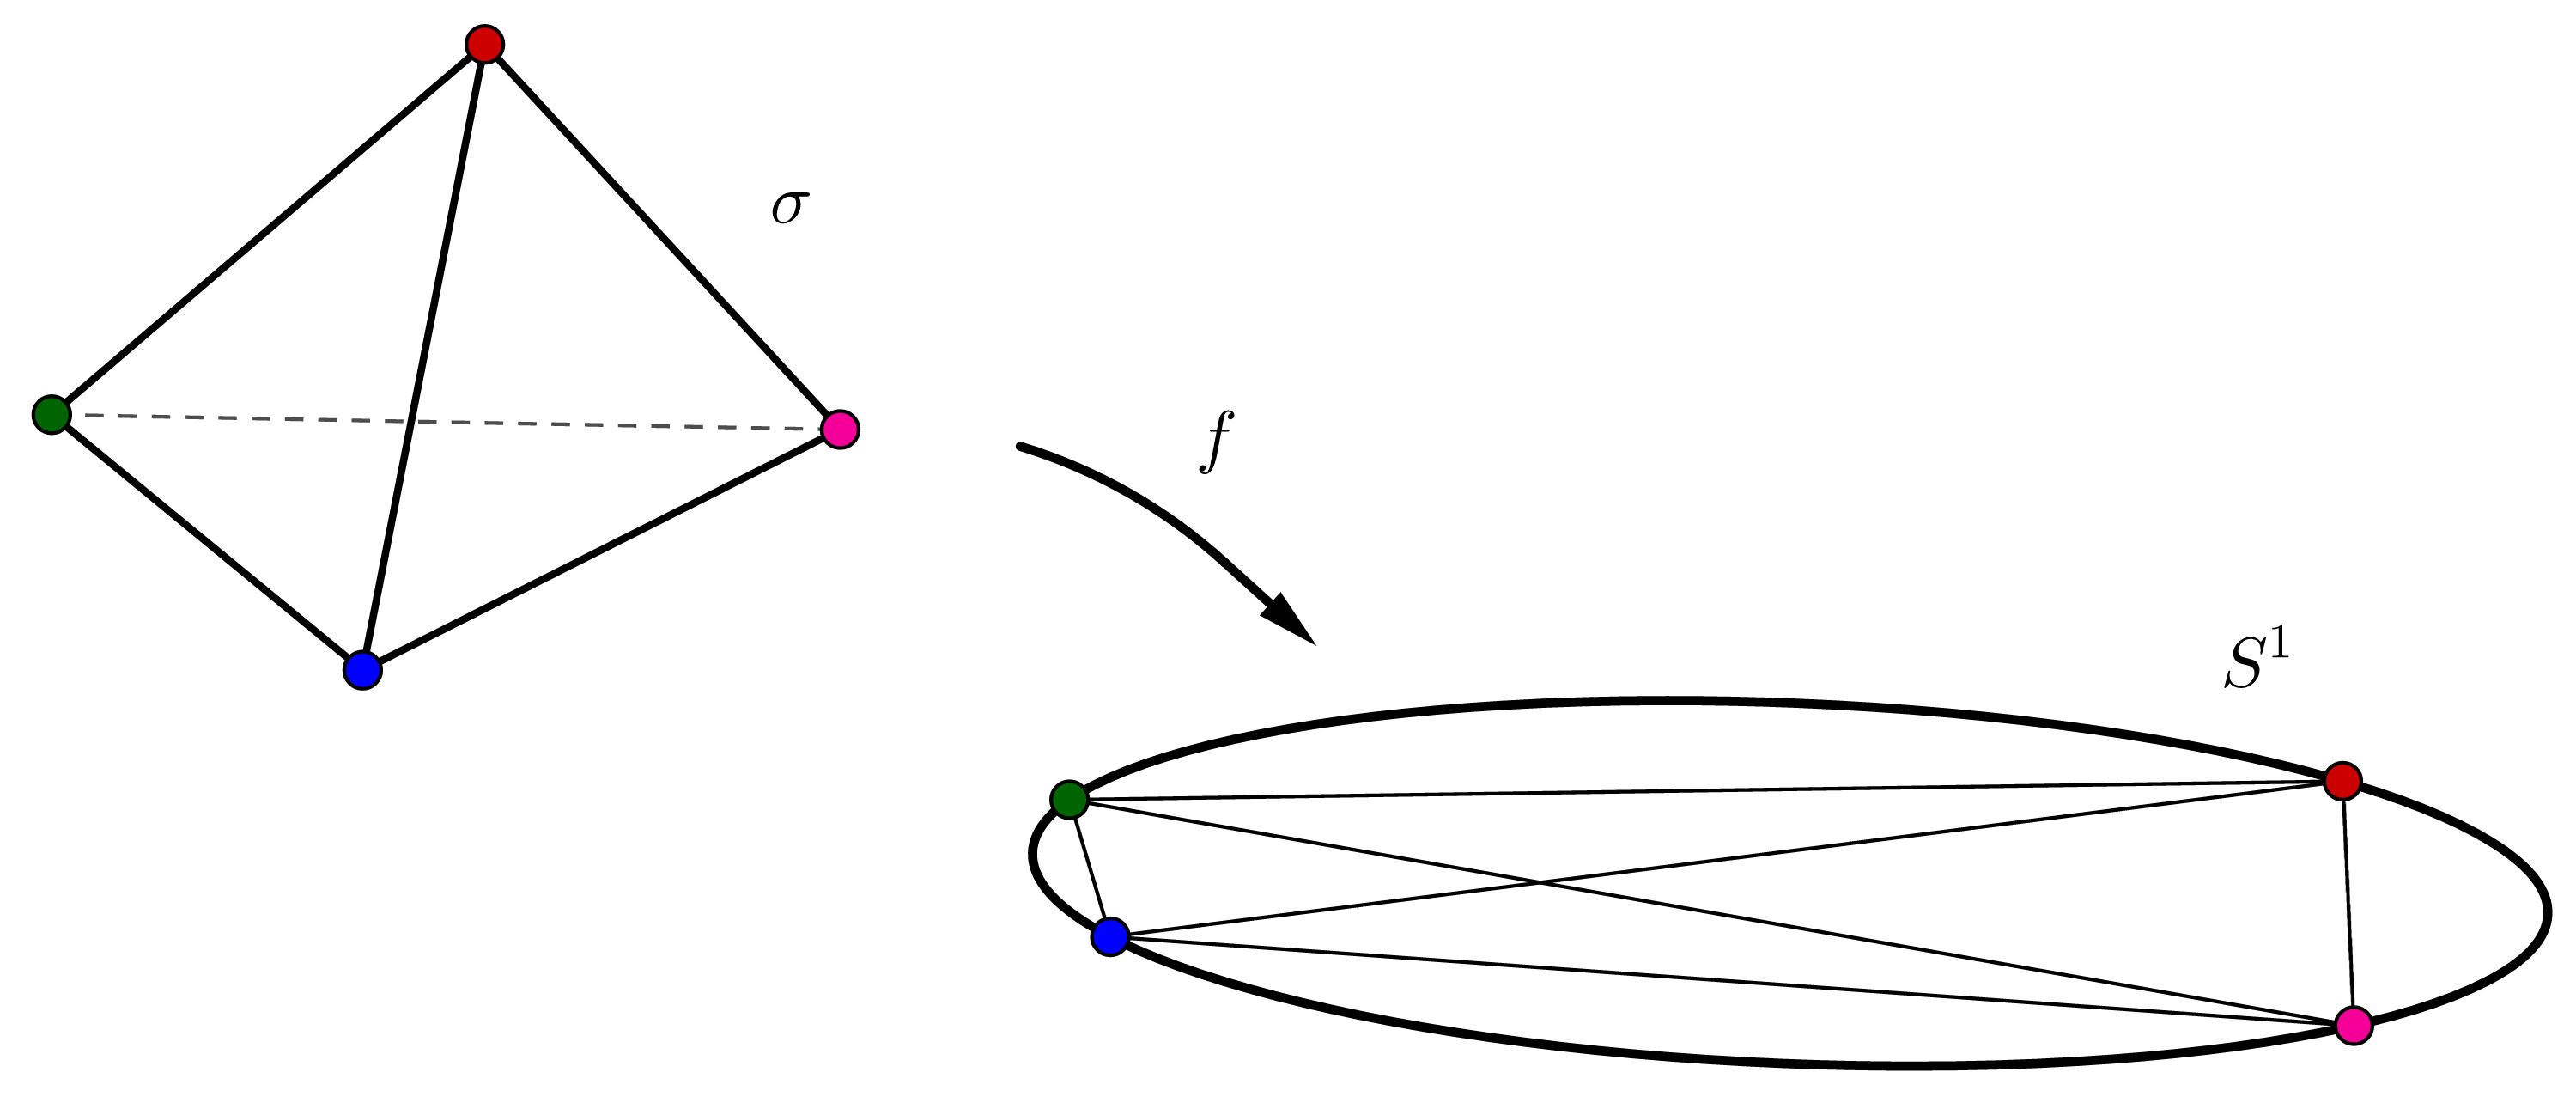
\includegraphics[width=0.9\textwidth]{figures/standard-position.png}
	\caption{
		\textbf{A tetrahedron $\sigma$ projected to the plane in standard position through a subdividing map $f$.}
		The four vertices of $\sigma^0$ map to the unit circle in the plane, thus form a convex arrangement.
		Four of the six edge of $\sigma^1$ map to the boundary of $f(\sigma)$, connecting $f(\sigma^0)$.
		The last two edges map across $f(\sigma)$, forming an intersection interior to $f(\sigma)$.
		Each vertex of the arrangement is essential in forming the convex hull of $f(\sigma^0)$.
	}
	\label{fig:standard-position}
\end{figure}